\section{The Dataset: NE15-MNIST}
\label{sec:data}
%Experiment setup/ collection method/ properties of each class/ etc.
The name of the first proposed dataset in the benchmarking system is NE15-MNIST which stands for Neuromorphic Engineering 2015 on MNIST.
The original MNIST dataset is downloaded from the website\footnote{http://yann.lecun.com/exdb/mnist/} of THE MNIST DATABASE of handwritten digits~\citep{lecun_gradient-based_1998}.
The NE15-MNIST is converted into a spiking version of the original dataset consisting of four subsets which were generated for different purposes:
\begin{itemize}
	\item \textit{Poissonian}
	to benchmarking existing methods of rate-based spiking models.
	\item \textit{FoCal}
	to promote the study of spatio-temporal algorithms applied to recognition tasks using few input spikes.
	\item \textit{DVS recorded flashing input}
	to encourage research on fast recognition methods which are found in the primate visual pathway.
	\item \textit{DVS recorded moving input}
	to trigger the study of algorithms targeting on continuous input from real-world sensors and to implement them on mobile neuromorphic robots.
\end{itemize}
The dataset can be found in the GitHub repository at: https://github.com/qian-liu/benchmarking.
\subsection{File~Formats}
	
Two file formats are supported in the dataset: jAER format~\citep{delbruck2008frame} (.dat or .aedat), and binary file in NumPy .npy format.
The  address event representation (AER) interface has been widely used in neuromorphic systems, especially for vision sensors.
The spikes are encoded as time events with corresponding addresses to convey information.
The spikes in jAER format, both recorded from a DVS retina and artificially generated, can be displayed in jAER software.
Fig~\ref{Fig:jaer} is a snapshot of the software displaying an .aedat file which is recorded by a DVS retina~\citep{serrano-gotarredona_128_2013}.
The resolution of the DVS recorded data is 128$\times$128.
%, while the original MNIST data is 28$\times$28.
The other format of spikes used is a list of spike source arrays in PyNN~\citep{davison2008pynn}, a description language for building spiking neuronal network models.
Python code for converting one file format to and from the other is also provided.

\begin{figure}[hbt]
  \centering
  \subfloat[A snapshot of jAER playing the DVS recorded spikes.]{
    \label{Fig:jaer}
    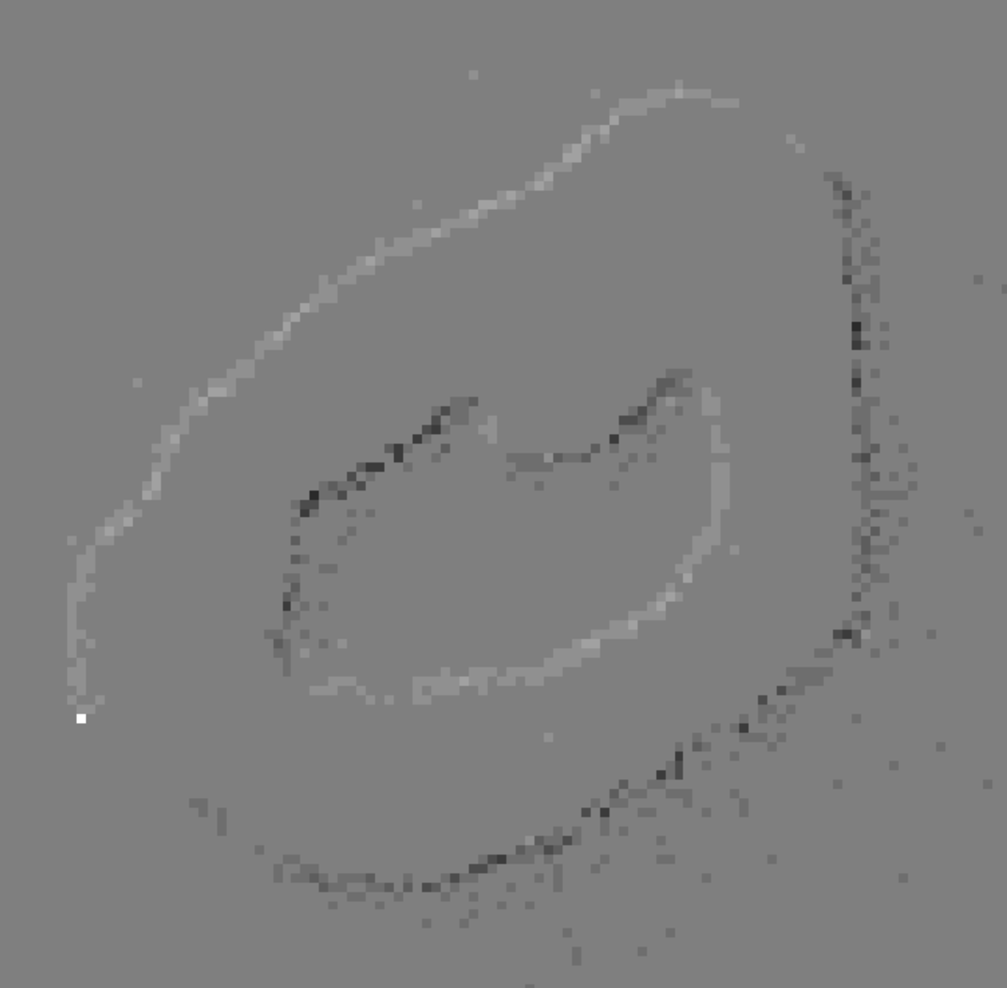
\includegraphics[width=0.22\textwidth]{images/dvs-128.pdf}
  }
  \subfloat[A snapshot of jAER playing Poissonian spike trains.]{
    \label{Fig:poisson}
    
\includegraphics[width=0.22\textwidth]{images/zero-28-2.pdf}
  }\\
  \subfloat[The raster plot of the Poissonian spike trains.]{
    \label{Fig:raster}
    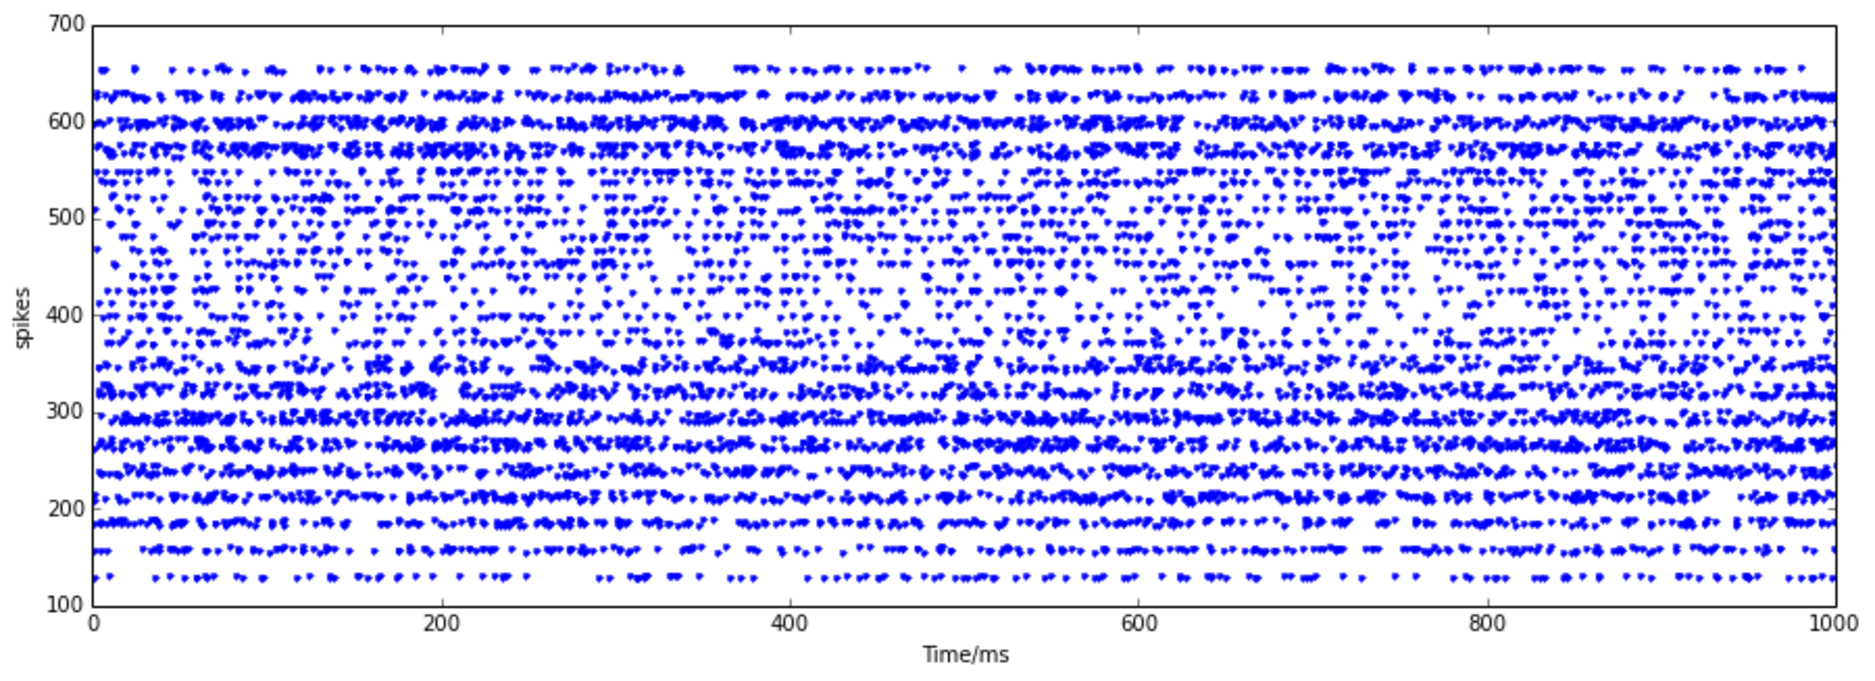
\includegraphics[width=0.48\textwidth]{images/zero.pdf}
  }
  
  \caption{Snapshots of jAER software playing spike presented videos. The same image of digit ``0'' are transform to spikes with two conventional means. The raster plot of the Poissonian spike trains is also provided.}
  \label{fig:zero}
\end{figure}

\subsection{Data Description}	
	\subsubsection{Poissonian}
	
	In the cortex, the timing of spikes is highly irregular~\citep{squire1998findings}.
	It can be interpreted that the inter-spike interval reflects a random process driven by the instantaneous firing rate.
	If the generation of each spike is assumed to be independent of all the other spikes, the spike train is seen as a Poisson process.
	The spiking rate can be estimated by averaging the pooled responses of the neurons.
		
	As stated above, rate coding is exclusively used in presenting images with spikes.
	The spiking rate of each neuron is in accordance with its corresponding pixel intensity.
	Instead of providing exact spike arrays, we share the Python code of generating the spikes.
	Every recognition system may require different spiking rates and various lengths of their durations.
	The generated Poissonian spikes can be in the formats of both jAER and PyNN spike source array.
	Thus, it is easy to visualise the digits and also to build spiking neural networks.
	Because different simulators generate random Poissonian spike trains with various mechanisms, languages and codes, using the same dataset enables performance evaluation on different simulators without the interference created by non-unified input.
	The same digit displayed in Fig~\ref{Fig:jaer} is converted to Poissonian spike trains, see Fig~\ref{Fig:poisson}.
	The raster plot can be found in Fig~\ref{Fig:raster}, indicating the intensities of the pixels.


	
	\subsubsection{Rank-Order-Encoding}
  A different way of encoding spikes is using a rank-order code; this means
keep just the order in which those spikes were fired and disregard the exact timing. Rank-ordered spike trains have been used in vision tasks under a biological plausibility constraint, making them a viable way of image encoding for neural applications~\citep{van2001rate,sen2009evaluating,masmoudi2010novel}.

Rank-ordered encoding can be performed using an algorithm known as 
{Filter overlap Correction algorithm} or FoCal~\citep{sen2009evaluating}. It models the foveal pit region, the highest resolution area of the retina, with four ganglion cell layers that show a{centre-surround behaviour~\citep{kolb2003retina}. In order to simulate these layers, four discrete 2D convolutions are performed. The centre-surround behaviour of the ganglion cells is modelled using Differences of Gaussians~(DoG). 
\begin{equation}
\label{eq-dog}
DoG_w(x,y) = \pm\frac{1}{2\pi\sigma_{w,c}^2}e^{\frac{-(x^2 + y^2)}{2\sigma_{w,c}^2}}
\mp\frac{1}{2\pi\sigma_{w,s}^2}e^{\frac{-(x^2 + y^2)}{2\sigma_{w,s}^2}}
\end{equation}
where $\sigma_{w,c}$ and $\sigma_{w,s}$ are the standard deviation for the 
centre and surround components of the DoG at layer $w$. The signs 
will be ($-$,$+$) if the ganglion cell has an OFF-centre behaviour and 
($+$,$-$) if it has an ON-centre one. Table~\ref{tab-kernel-specs} 
describes the parameters used to compute the convolution kernels at each 
scale $w$.

\begin{table}[htb]
 \caption{Simulation parameters for ganglion cells}
  \begin{center}


  \bgroup
  \def\arraystretch{1.4}
      
  \begin{tabular}{c c c c c c}
    \begin{minipage}{0.7cm}\centering Layer \end{minipage}& 
    \begin{minipage}{0.8cm}\centering Centre \\type \end{minipage}& 
    \begin{minipage}{0.7cm} \centering Matrix width \end{minipage}&  
    \begin{minipage}{1.3cm}\centering Centre std. dev. ($\sigma_c$)\vspace*{0.1cm}\end{minipage} & 
    \begin{minipage}{1.3cm}\centering Surround std. dev. ($\sigma_s$)\vspace*{0.1cm}\end{minipage} & 
    \begin{minipage}{1.3cm}\centering Sampling resolution (cols,rows)\vspace*{0.1cm}\end{minipage} \\
    \hline
    \begin{minipage}{0.7cm}\centering 1  \end{minipage} &
    \begin{minipage}{0.8cm}\centering OFF \vspace*{0.005cm} \end{minipage}& 
    \begin{minipage}{0.7cm}\centering$3$ \end{minipage}& 
    $0.8$ & $6.7 \times \sigma_c$ &  1, 1 \\
    \begin{minipage}{0.7cm}\centering 2 \end{minipage} & 
    \begin{minipage}{0.8cm}\centering ON \vspace*{0.005cm}\end{minipage} & 
    \begin{minipage}{0.7cm}\centering $11$ \end{minipage}& 
    $1.04$ & $6.7 \times \sigma_c$ & 1, 1 \\
    \begin{minipage}{0.7cm}\centering3 \end{minipage} &
    \begin{minipage}{0.8cm}\centering OFF \vspace*{0.005cm}\end{minipage} & 
    \begin{minipage}{0.7cm}\centering $61$ \end{minipage}& 
    $8$ & $4.8 \times \sigma_c$ & 5, 3 \\
    \begin{minipage}{0.7cm}\centering 4  \end{minipage} & 
    \begin{minipage}{0.8cm}\centering ON \vspace*{0.005cm}\end{minipage} & 
    \begin{minipage}{0.7cm}\centering $243$\end{minipage} &
    $10.4$ & $4.8 \times \sigma_c$ & 5, 3 
  \end{tabular}
  \egroup
 \end{center}
  \label{tab-kernel-specs}
\end{table}

Every pixel value in the convolved images (Fig. \ref{fig-convolution-results}) 
is inversely proportional to a spike emission time (i.e. the higher the pixel value, the sooner the spike will be sent out.)

\begin{figure}[hbt]
  \centering
  \subfloat[Original image]{
    \label{sfig-rank-ordered-original}
    
\includegraphics[width=0.15\textwidth]{original_21-0}
  }
  \subfloat[Layer 1 (\textsc{off}-centre)]{
    \label{sfig-rank-ordered-midget-off}
    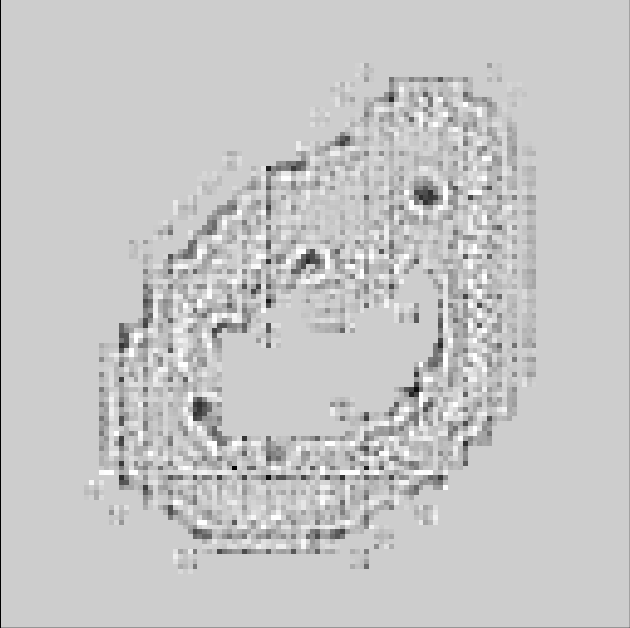
\includegraphics[width=0.15\textwidth]{filtered-21-0-layer-0}
  }
  \subfloat[Layer 2 (\textsc{on}-centre)]{
    \label{sfig-rank-ordered-midget-on}
    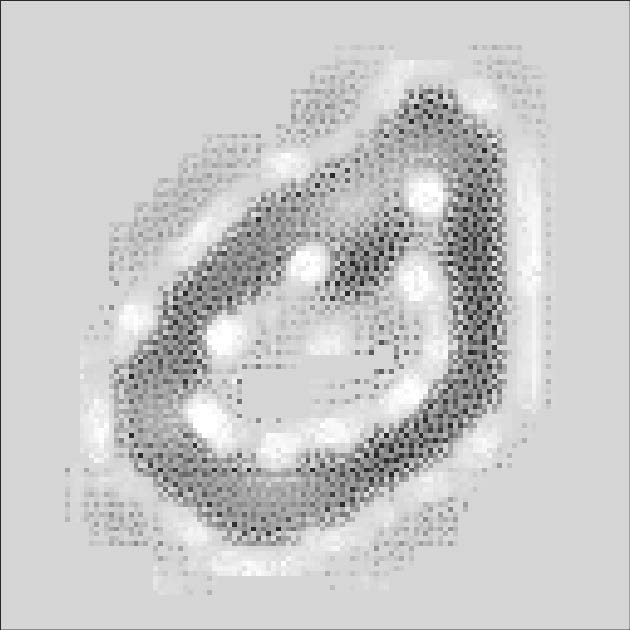
\includegraphics[width=0.15\textwidth]{filtered-21-0-layer-1}
  }\\
  \subfloat[Layer 3 (\textsc{off}-centre)]{
    \label{pic-lena-P-OFF}
    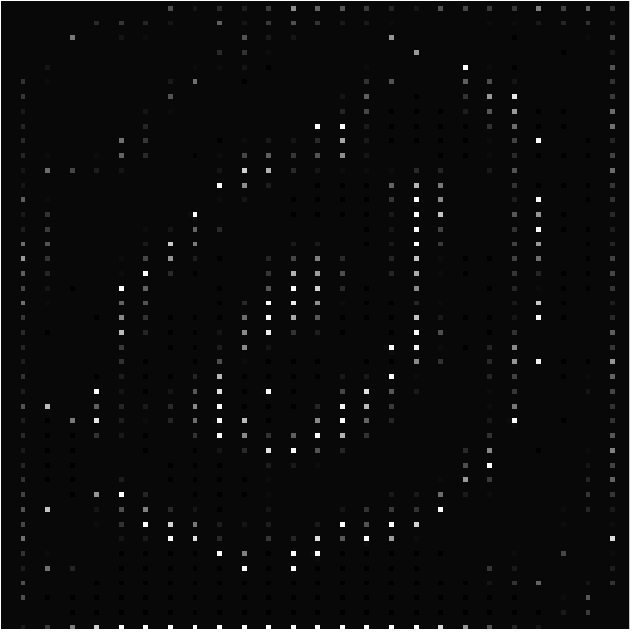
\includegraphics[width=0.15\textwidth]{filtered-21-0-layer-2}
  }
  \subfloat[Layer 4 (\textsc{on}-centre)]{
    \label{pic-lena-P-ON}
    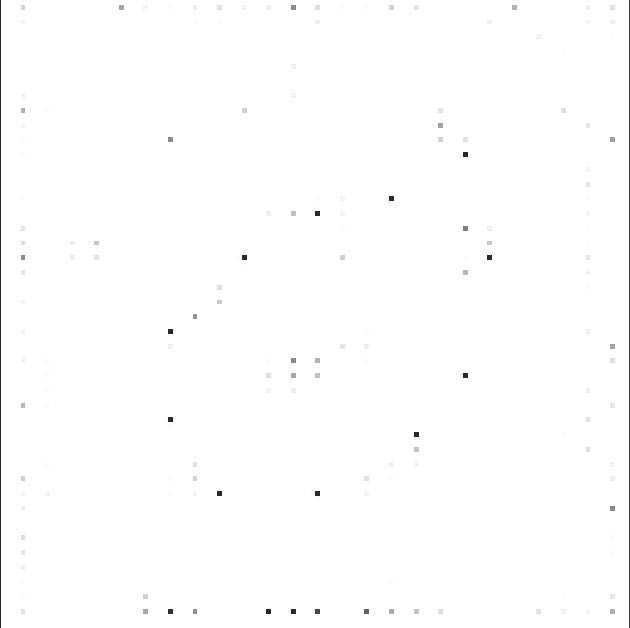
\includegraphics[width=0.15\textwidth]{filtered-21-0-layer-3}
  }
  \caption{Results of correcting the spikes from the simulated ganglion cell layers.}
  \label{fig-convolution-results}
\end{figure}
The algorithm also performs a redundancy correction step, it does so by 
adjusting the convolved image's pixel value according to the correlation 
between convolution kernels (Alg.~\ref{code-focal-corr}).
\begin{algorithm}[h]
  \caption{FoCal, Part 2}
  \label{code-focal-corr}
  \begin{algorithmic}
    \Procedure{Correction}{coeffs $C$, correlations $Q$}
    \State $N \leftarrow \emptyset$ \Comment{Corrected coefficients}
    \Repeat
    \State $m \leftarrow max(C)$\Comment{Obtain maximum from $C$}
    \State $M \leftarrow M \cup m$\Comment{Add maximum to $M$}
    \State $C \leftarrow C \setminus m$\Comment{Remove maximum from $C$}
    \ForAll{$ c \in C$} \Comment{Adjust all remaining $c$}
    \If{$Q(m, c) \neq 0$} \Comment{Adjust only near}
    \State $c \leftarrow c - m \times Q(m, c)$
    \EndIf
    \EndFor
    \Until{$C = \emptyset$}
    \State \textbf{return} $M$
    \EndProcedure
  \end{algorithmic}
\end{algorithm}

<<<<<<< HEAD
After the correction step, the most important information can be recovered using only the first 30\% of the spikes~\citep{sen2009evaluating}. These significant spikes are shown in Fig.~\ref{fig-raster-plot-30pc}, assuming that each spike will be generated 1~ms apart. Neurons in Layer 1 emit spikes faster and in larger quantities than any other layer, making it the most important one. Layers 2 and 3 have few spikes, this is due to the large convolution kernels used to simulate the ganglion cells. One of the main advantages of ROC is that neurons will only spike once, this can be seen particularly well in these two layers. Layers 0 and 1 encode fine details, while layers 2 and 3 result in blob like features.
\begin{figure}[hbt]
  \centering
      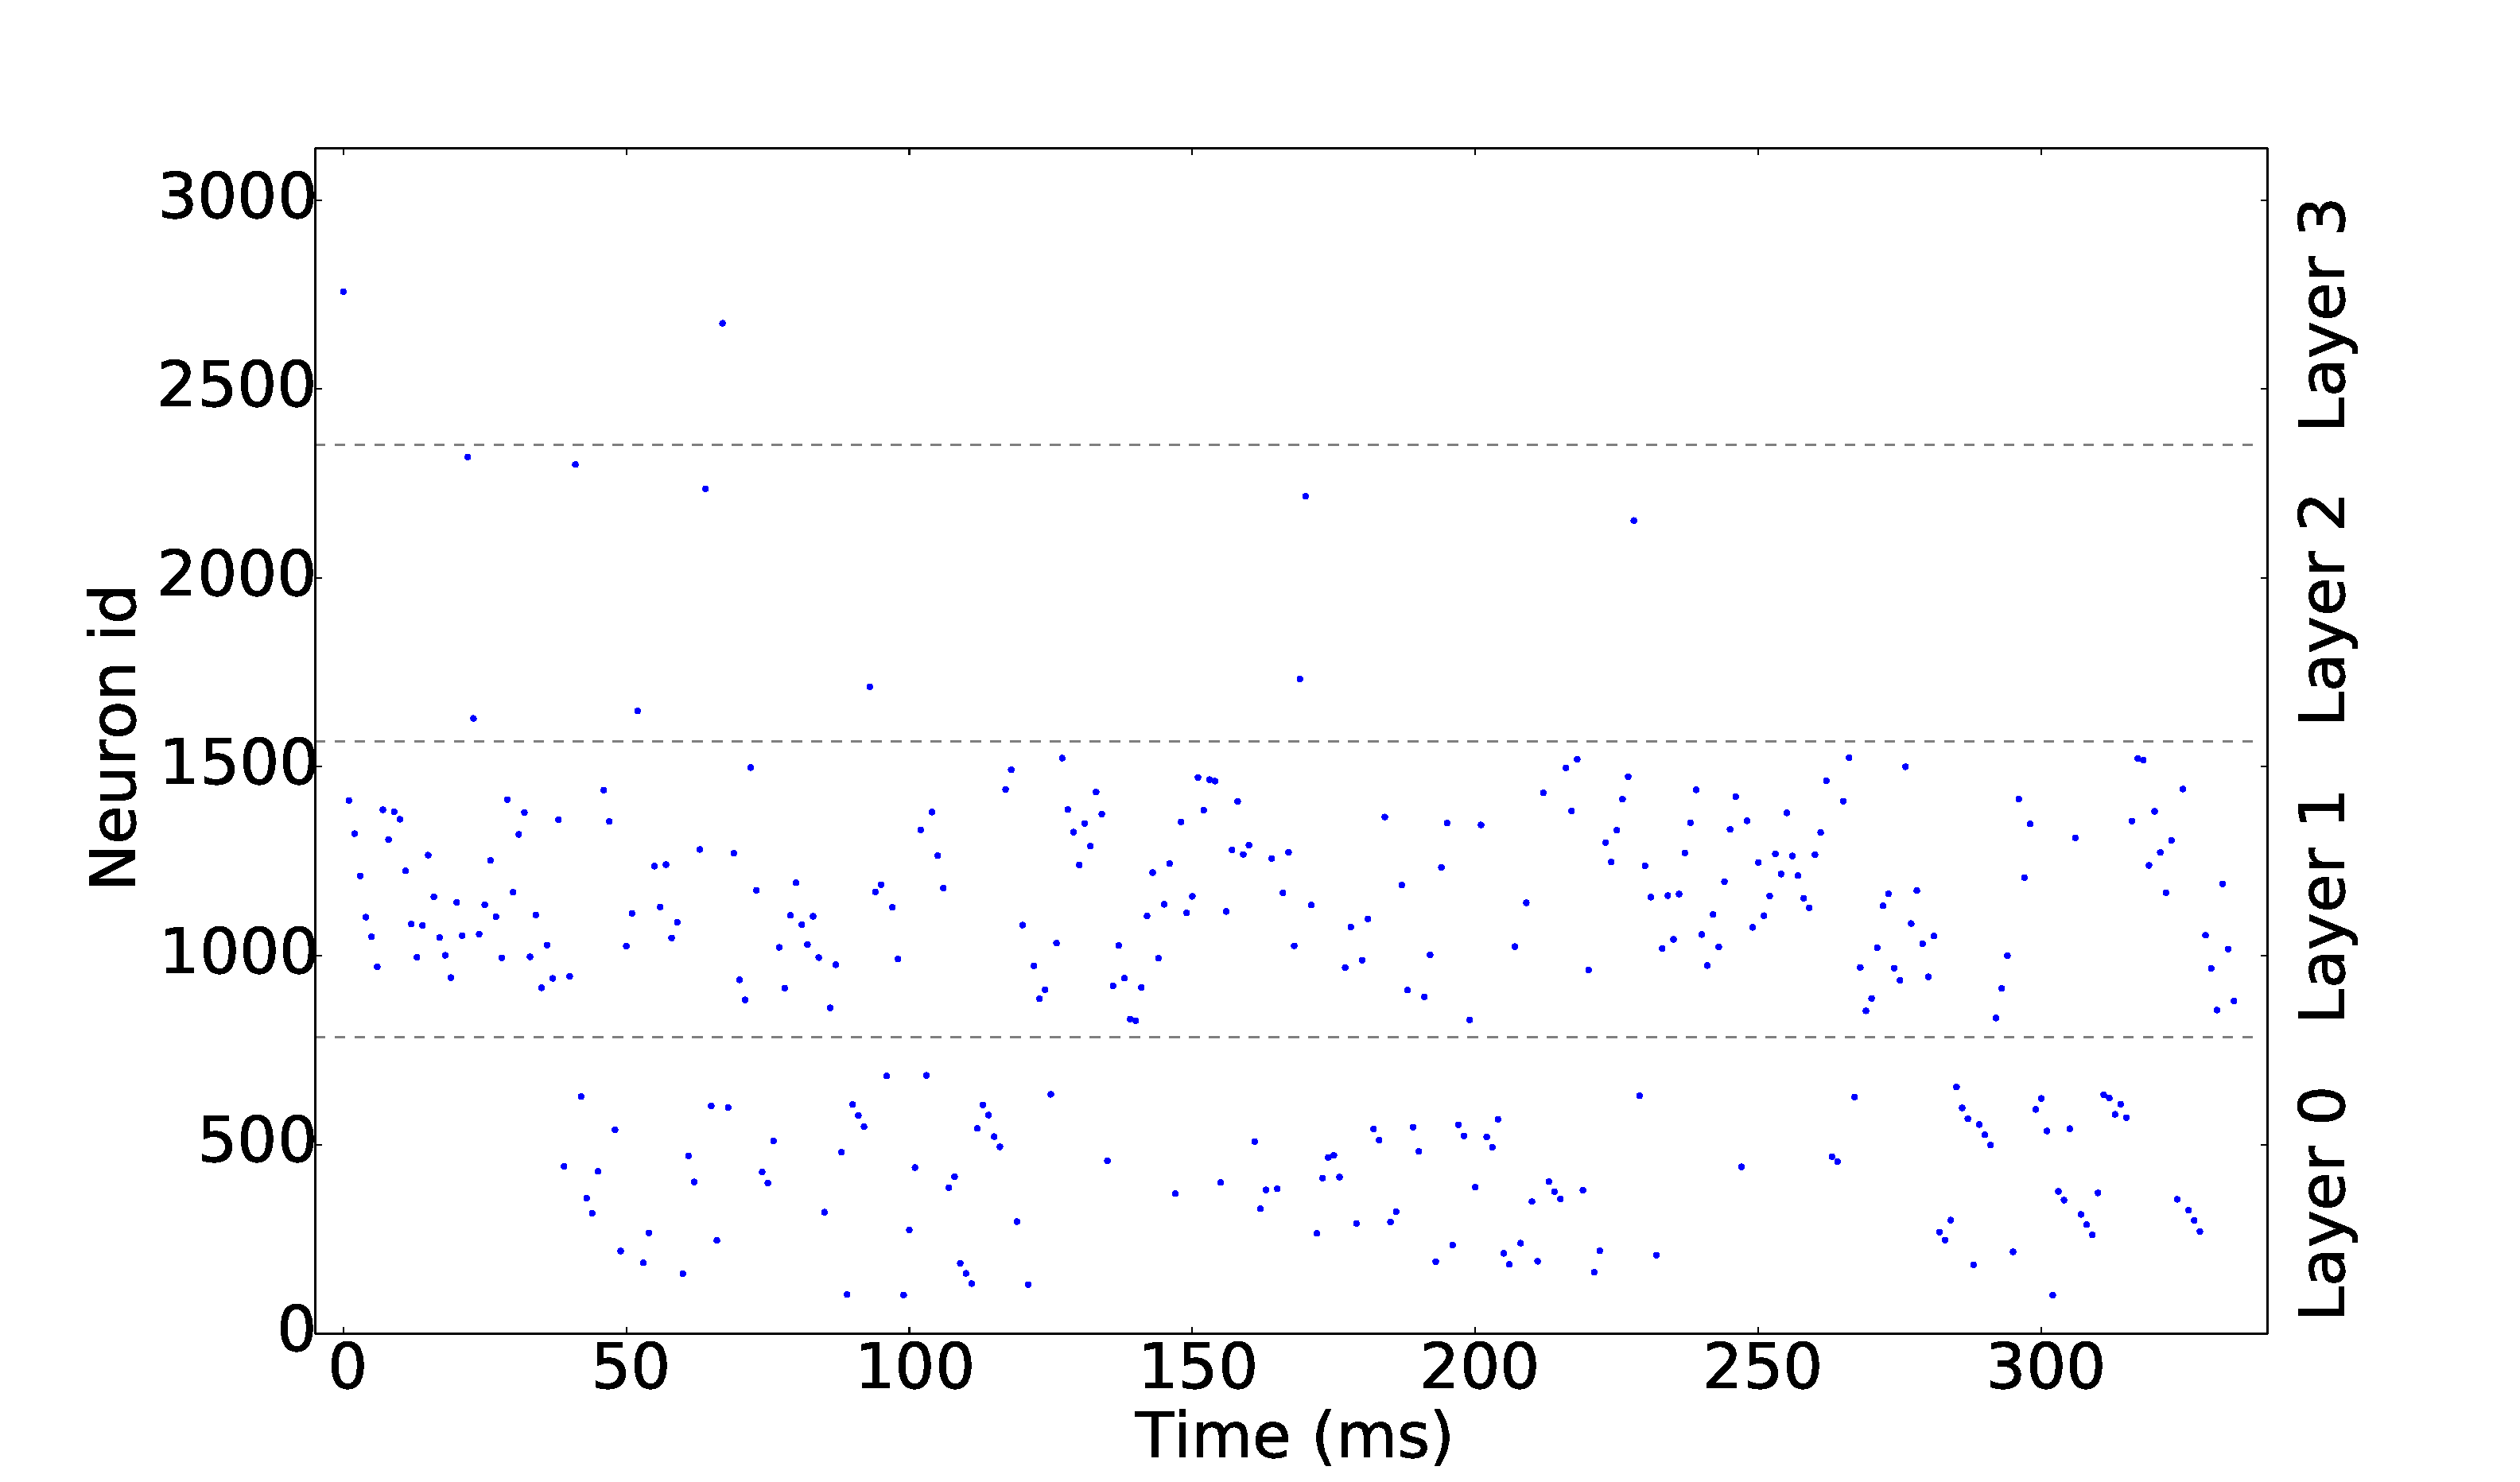
\includegraphics[width=0.475\textwidth]{raster-plot-21-0-30pc}
      \caption{First 30\% of the rank-order encoded spikes produced with FoCal.}
      \label{fig-raster-plot-30pc}
=======
After the correction step, the most important information can be recovered using only the first 30\% of the spikes~\citep{basab-model}. These significant spikes are shown in Fig.~\ref{fig-raster-plot-30pc}, assuming that each spike will be generated 1~ms apart. Neurons in Layer 1 emit spikes faster and in larger quantities than any other layer, making it the most important one. Layers 2 and 3 have few spikes, this is due to the large convolution kernels used to simulate the ganglion cells. One of the main advantages of ROC is that neurons will only spike once, this can be seen particularly well in these two layers. Layers 0 and 1 encode fine details, while layers 2 and 3 result in blob like features.

\begin{figure}[hbt]
  \centering
    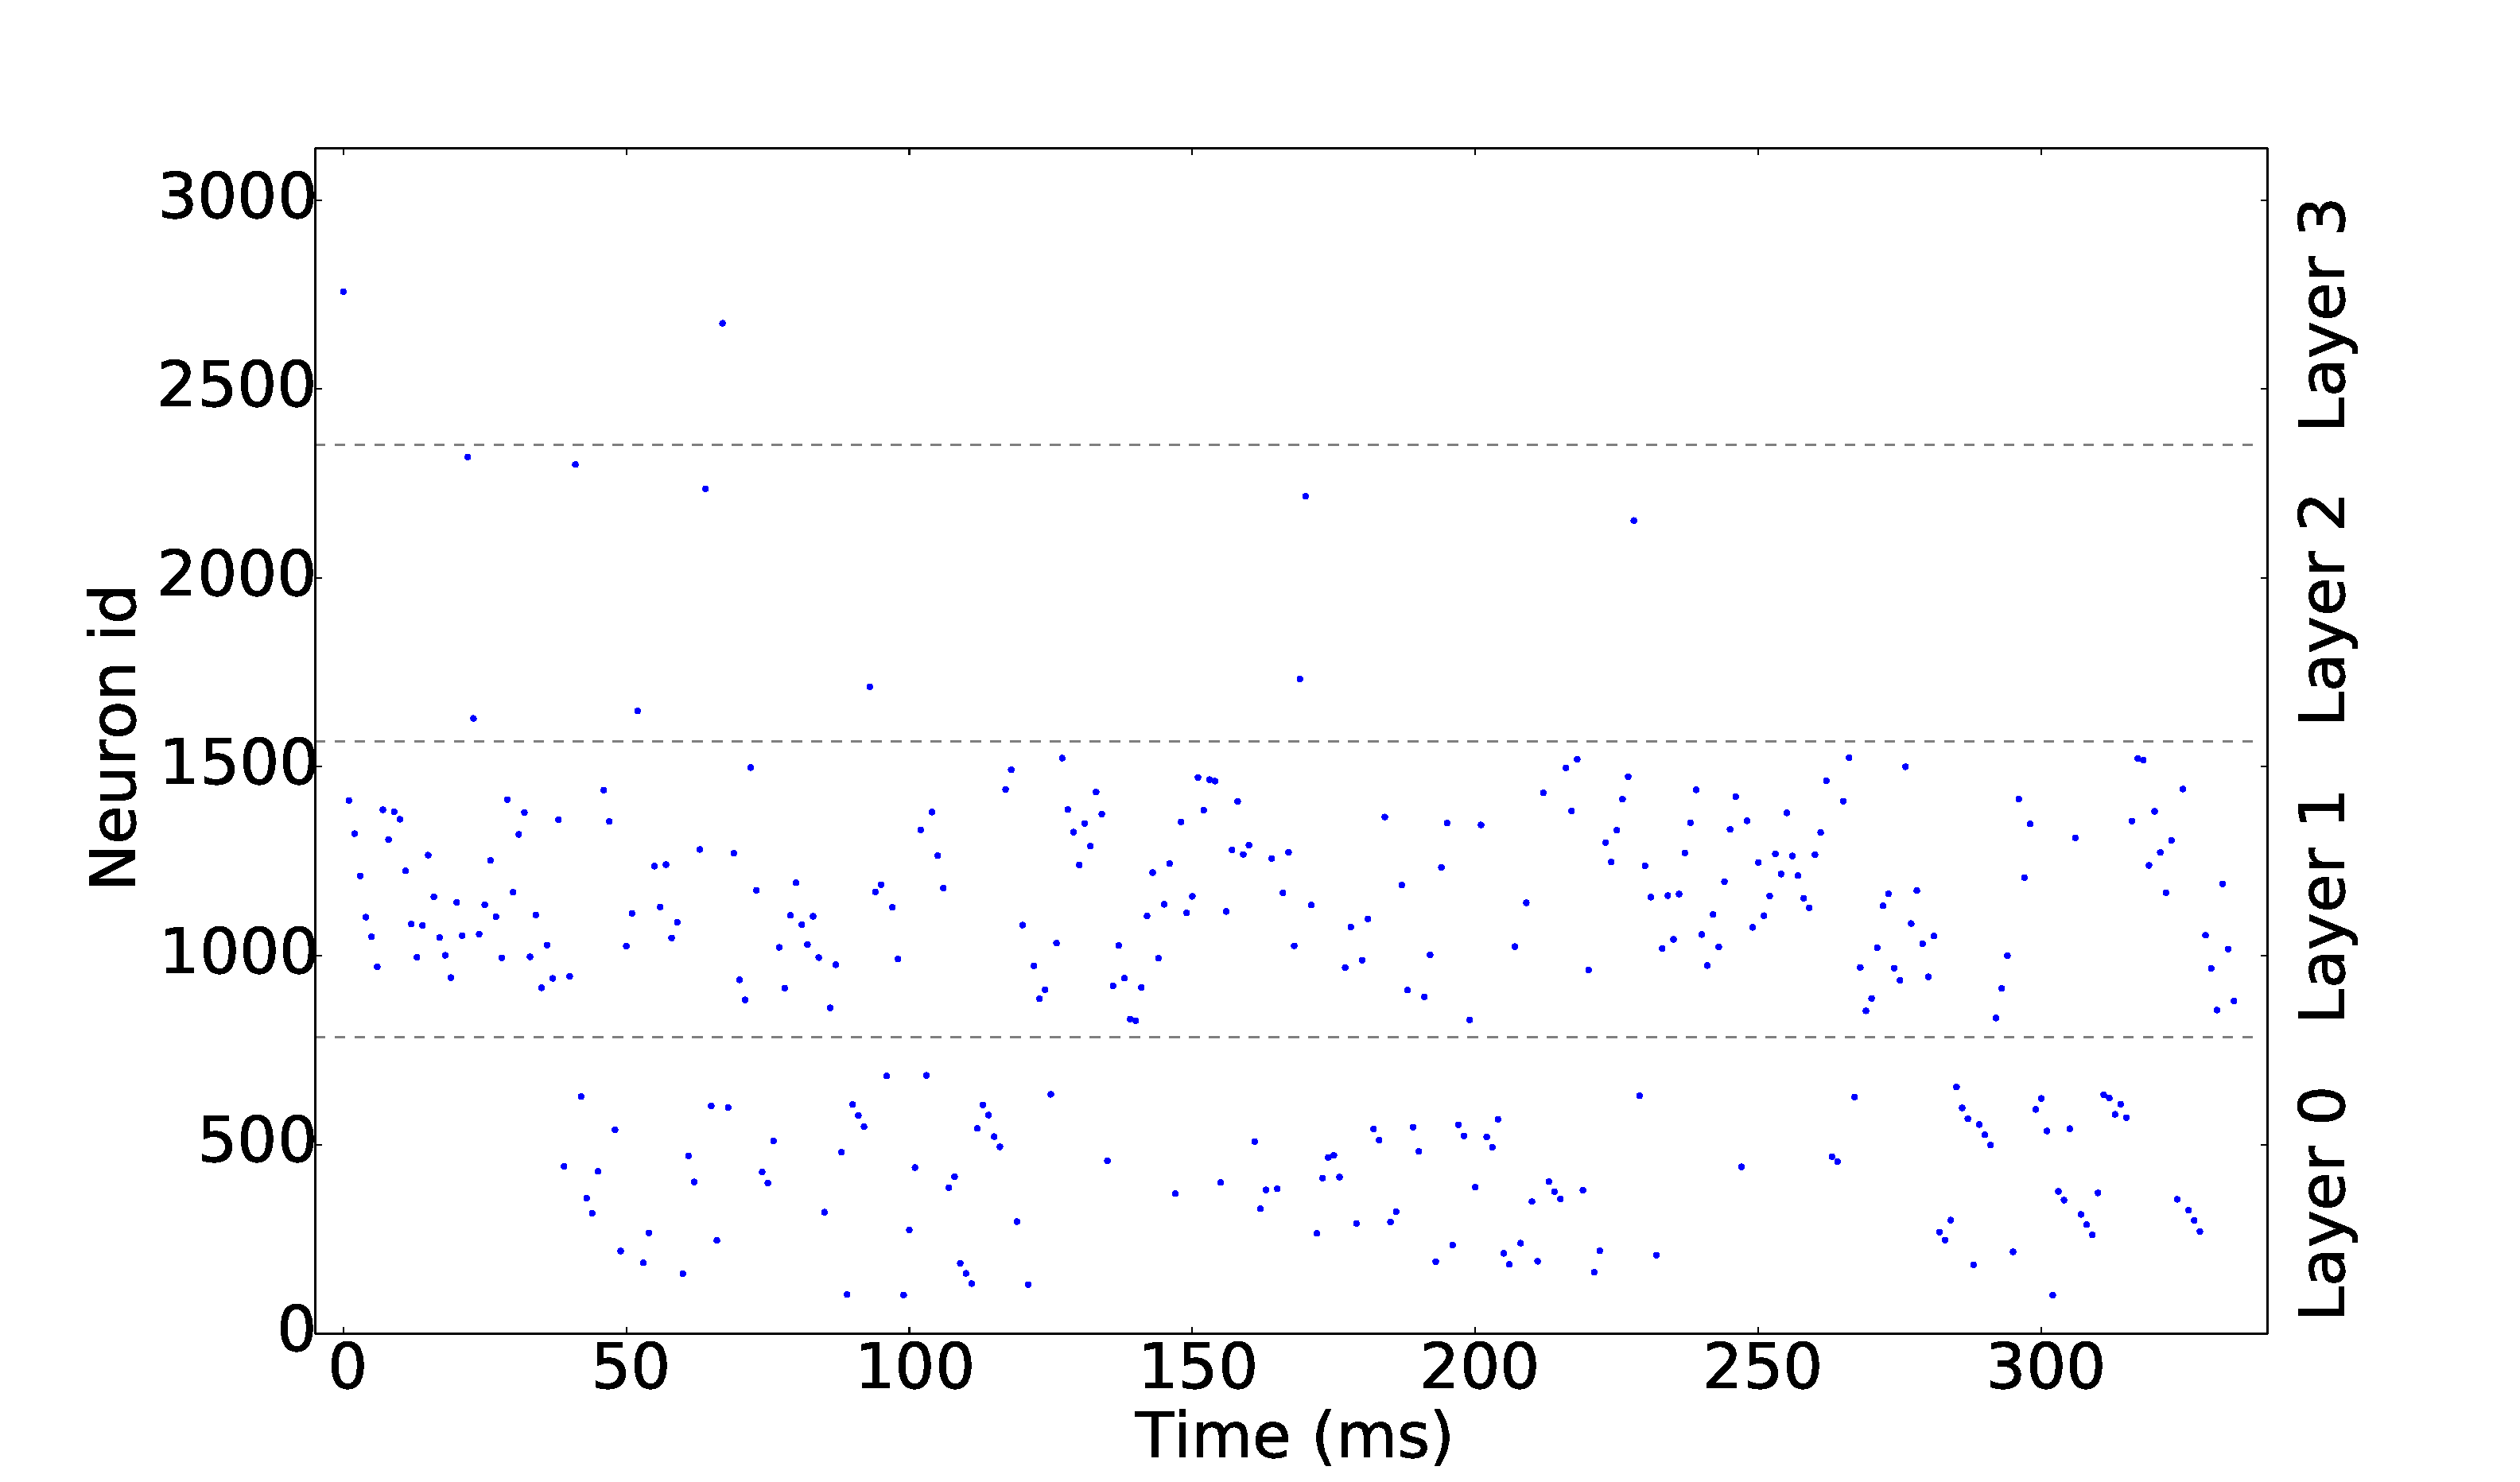
\includegraphics[width=0.475\textwidth]{raster-plot-21-0-30pc}
%    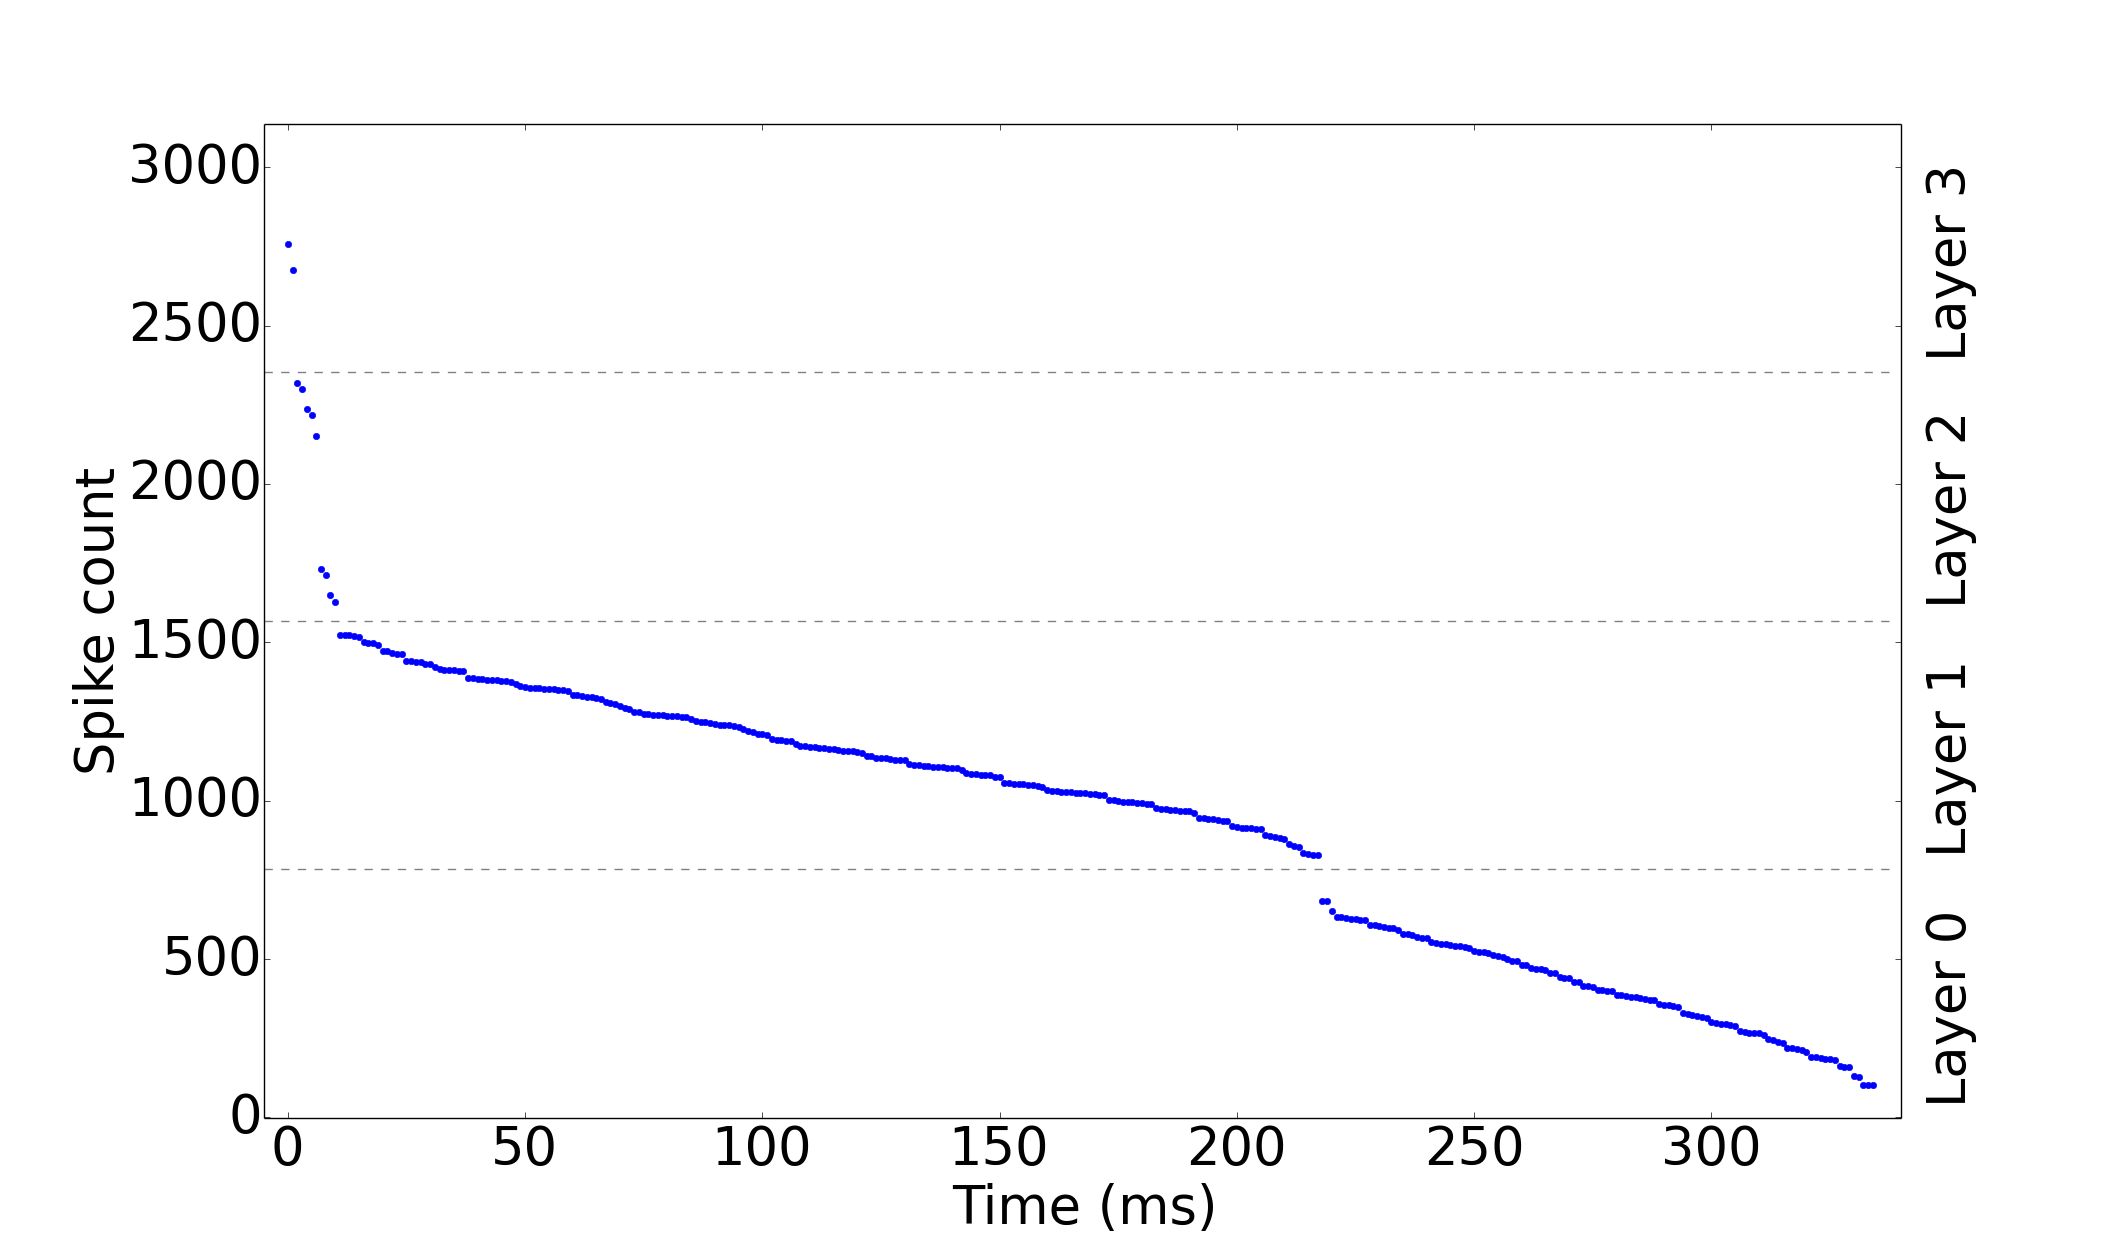
\includegraphics[width=0.475\textwidth]{sorted-raster-plot-21-0-30pc}
  \caption{First 30\% of the rank-order encoded spikes produced with FoCal.}
  \label{fig-raster-plot-30pc}
>>>>>>> 7059eb97ce659e6943f936f858bc9f8504ba0a63
\end{figure}

Figure \ref{fig-reconstruction-results} shows the reconstruction results for the two stages of the algorithm. On Fig. \ref{pic-lena-reconstructed-raw} the reconstruction was applied after the convolution, a blurry image is the result of redundancy in the spike representation. A better reconstruction can be obtained after Algorithm \ref{code-focal-corr} has been applied, the result is shown in Figure \ref{pic-lena-reconstructed-focal}.


\begin{figure}[hbt]
  \centering
  \subfloat[Original image]{
    \label{sfig-rank-ordered-original-1}
    
\includegraphics[width=0.15\textwidth]{original_21-0}
  }
  \subfloat[No correction]{
    \label{pic-lena-reconstructed-raw}
    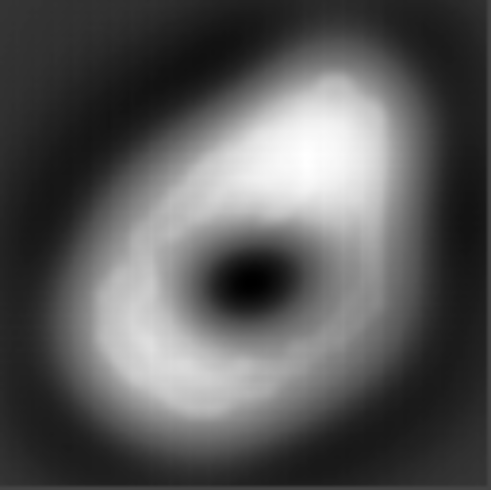
\includegraphics[width=0.15\textwidth]{reconstructed_21-0_raw}
  }
  \subfloat[FoCal]{
    \label{pic-lena-reconstructed-focal}
    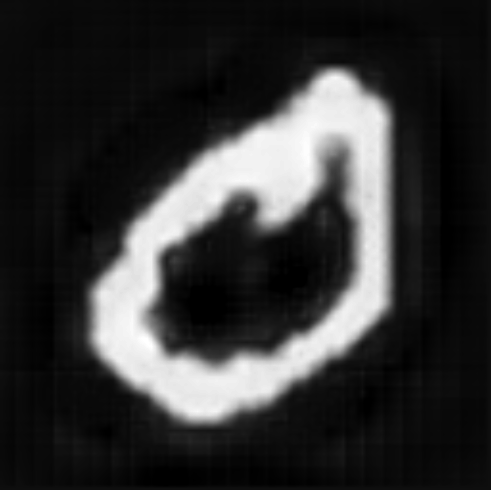
\includegraphics[width=0.15\textwidth]{reconstructed_21-0_100pc}
  }
  \caption{Reconstruction result comparison.}
  \label{fig-reconstruction-results}
\end{figure}
%Two resolutions are provided for the rank-order encoded portion of the database, the first is the original $28\times28$ one. An additional up-scaled resolution version is also provided, the images where scaled to a $128\times128$ resolution using bi-cubic interpolation, this was done to match the DVS native resolution. 

The source Python scripts to transform images to ROC spike trains, to convert the results into AER and PyNN's spike source array can be found in the dataset's website.
	\subsubsection{DVS Sensor Output with Flashing Input}
	\label{subsec_flash}
	The purposes of including the subset of DVS recorded flashing digits are to promote the application of Rank-Order-Coding to DVS output, and accelerate the fast on-set recognition by using just the beginning part of spike trains within less than 30~ms.
	
	Each digit and a blank image were shown alternately and each display lasted one second.
	The digits were displayed on a LCD monitor in front of the DVS retina~\citep{serrano-gotarredona_128_2013} and were placed in the centre of the visual field of the camera.
%	Each recording was cut into 10 sub sections.
	Since there are two polarities of the spikes: 'ON' indicates the increase of the intensity while 'OFF' reflects the opposite, there are an 'ON' and an 'OFF' flashing recordings respectively per digit.
	In Fig~\ref{fig:flash}, the bursty of the spikes is illustrated where most of the spikes occur in a 30~ms slot. 
	In total, the subset of the database contains 2$\times$60000 recordings for training and 2$\times$10000 for testing.
%	Due to the size limit of online repositories, only the third of every sequence of flashes is published.

	\begin{figure}[b!]
	  \centering
	  \subfloat[Spikes recorded in the order of neuron ID during 1s of time.]{
	  	    \label{fig:flash_all}
	  	    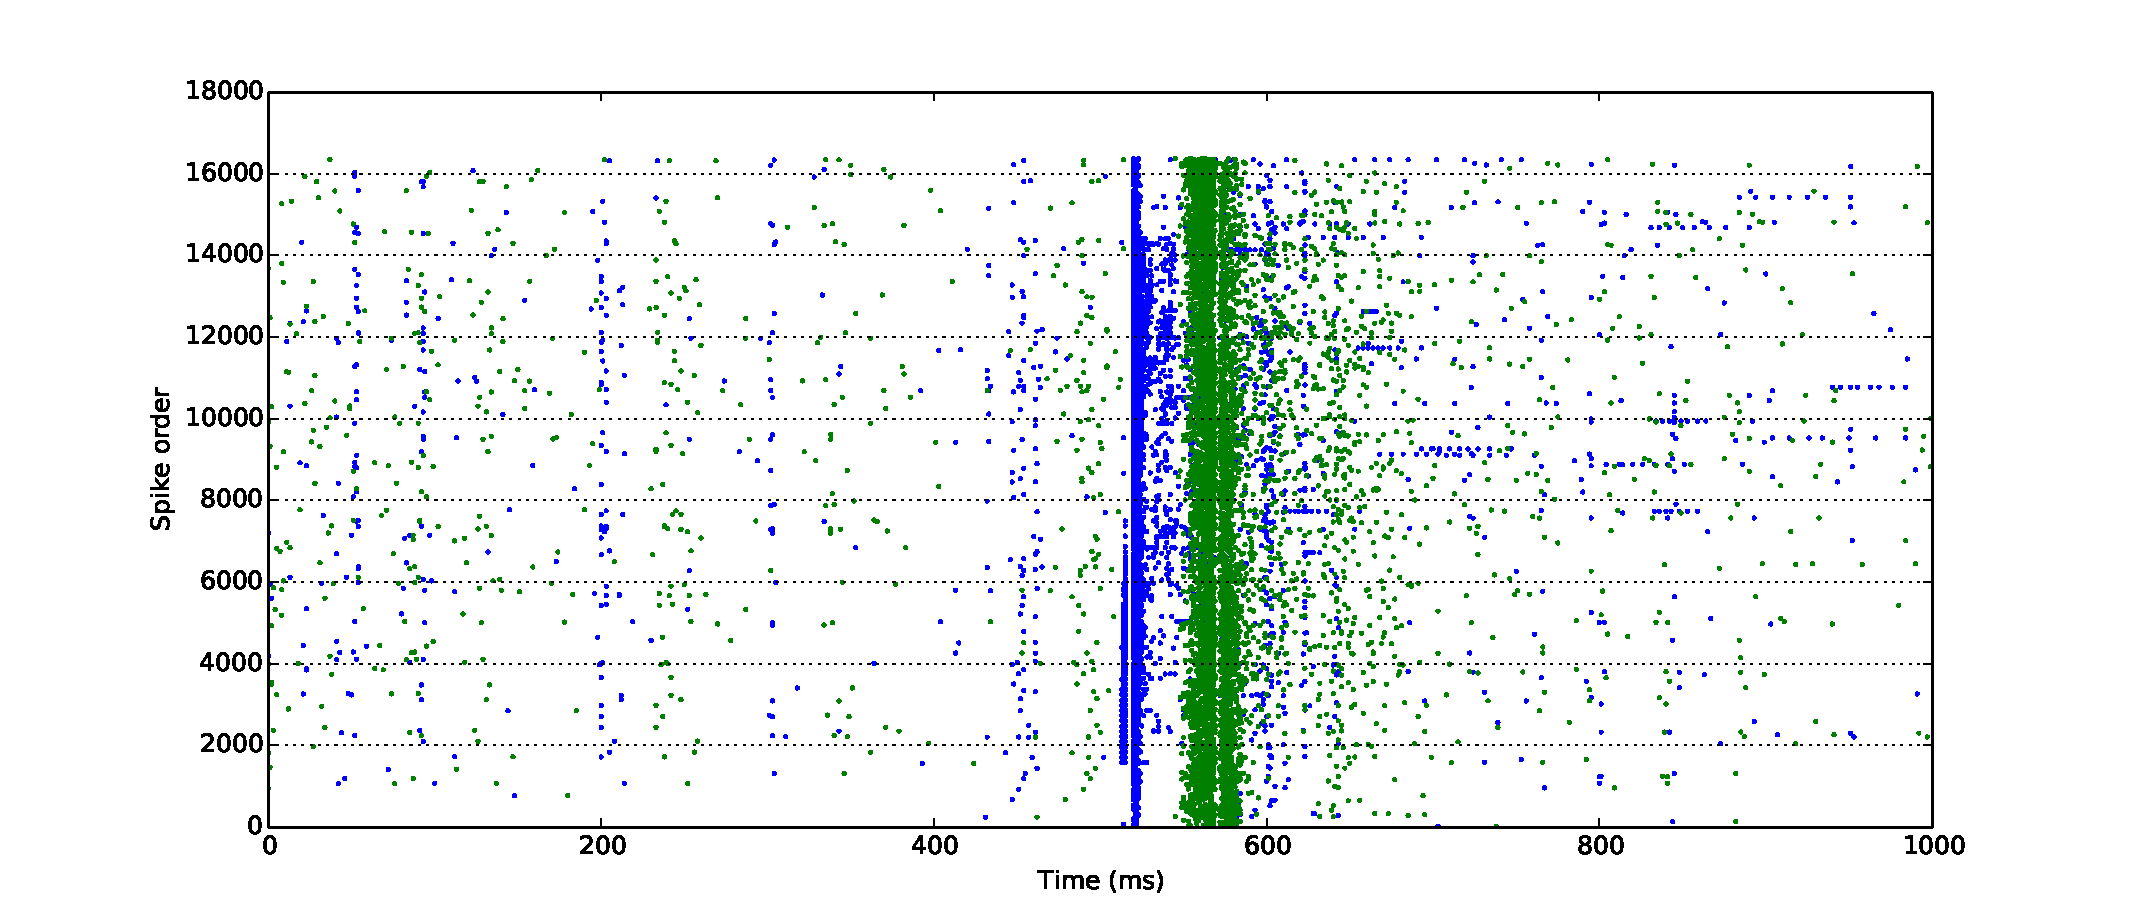
\includegraphics[width=0.48\textwidth]{flash_full.pdf}
	  	  }
	  	  \\
	  \subfloat[Spikes plotted in the sequence of appearing time during 1s of time. Bursty spikes apeer in slots less than 30~ms. ]{
	    \label{fig:flash_a}
	    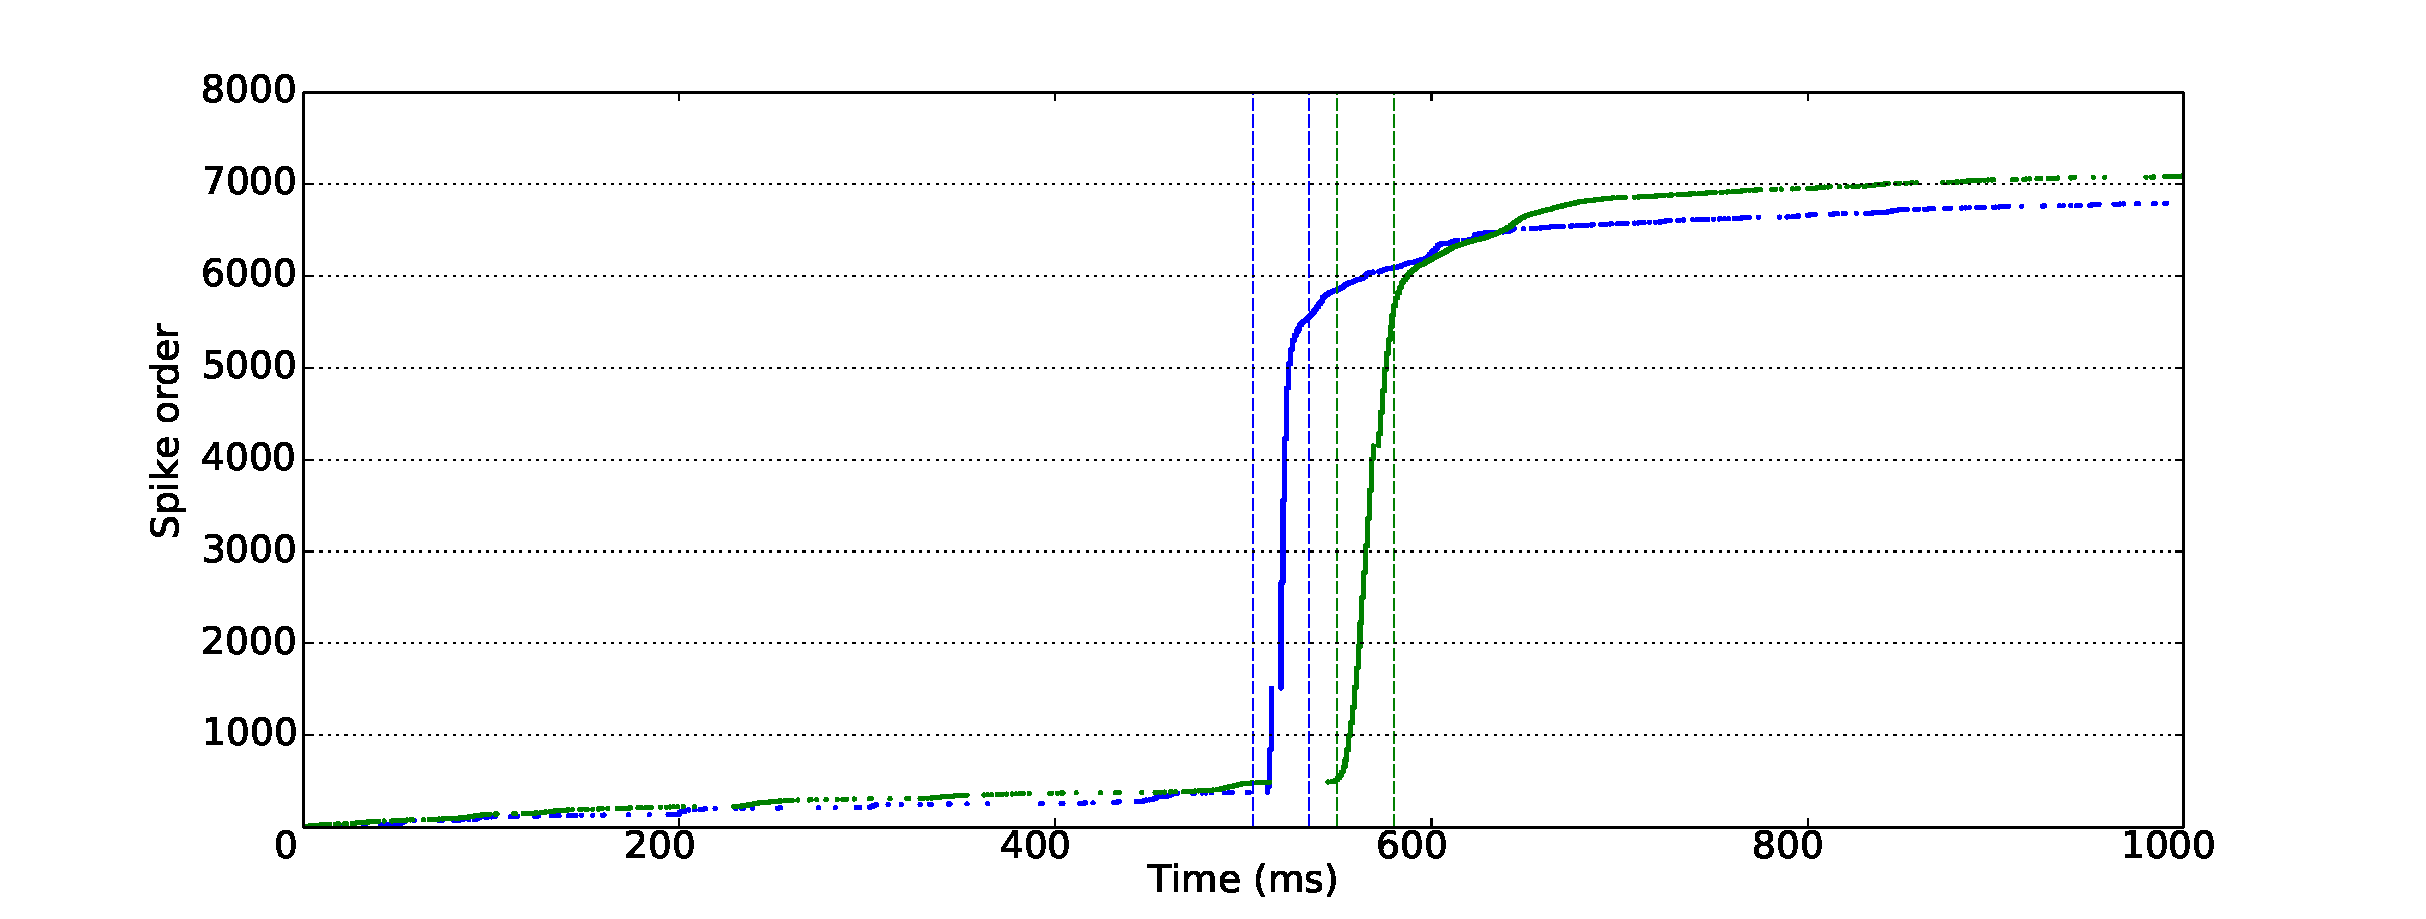
\includegraphics[width=0.48\textwidth]{flash_full_order.pdf}
	  }
%	  \\
%	  \subfloat[Bursty spikes appearing in a 30~ms slot.]{
%	  	\label{fig:flash_b}
%	  	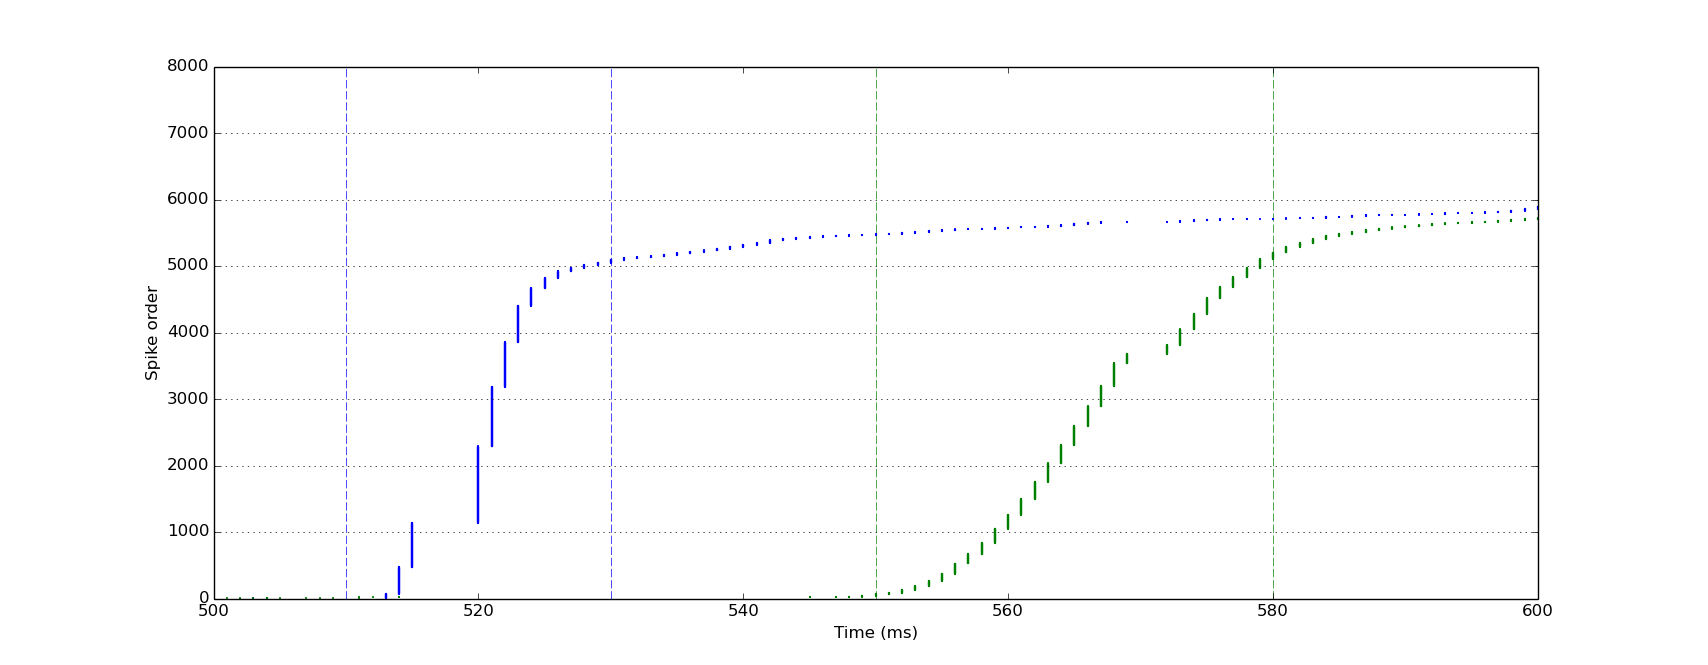
\includegraphics[width=0.48\textwidth]{flash_100.png}
%	  }

	  \caption{The bursty of spikes is illustrated where most of the spikes occur in a 30~ms slot. Blue for 'ON' events and green for 'OFF'.}
	  \label{fig:flash}
	\end{figure}
%	\subsubsection{DVS Sensor Output with Oscillating Input}
	\subsubsection{DVS Sensor Output with Moving Input}
	In order to address the problems of position- and scale- invariance, the subset of DVS recorded moving digits is presented.
	
	MNIST digits were scaled to three different sizes, by using smooth interpolation algorithms to increase their size from the original 28x28 pixel size, and displayed on the monitor with slow motion. 
	The same DVS~\citep{serrano-gotarredona_128_2013} used in Section~\ref{subsec_flash} captured the movements of the digits and generated spike trains for each pixel of its 128$\times$128 resolution.
	A total of 30,000 recordings were made: 10 digits, at 3 different scales, 1000 different handwritten samples for each.
%	The subset is available at the website\footnote {http://imse-cnm.csic.es/caviar/MNIST\_DVS}.
	